\documentclass{article}
\usepackage{graphicx} % Required for inserting images
\usepackage{hyperref}     % Per i link
\usepackage{array}        % Per tabelle con allineamento personalizzato
\usepackage{longtable}    % Per tabelle lunghe e ordinate
\usepackage{listings}    % Pacchetto per il codice
\usepackage{xcolor}      % Per la colorazione del codice
\usepackage{float}   

\lstset{
    language=Python,
    basicstyle=\ttfamily\small,  % Stile del testo
    keywordstyle=\color{blue},   % Colore delle parole chiave
    stringstyle=\color{red},     % Colore delle stringhe
    commentstyle=\color{gray},   % Colore dei commenti
    frame=single,                % Cornice intorno al codice
    numbers=left,                % Numeri di riga a sinistra
    numberstyle=\tiny\color{gray}
}

\title{Progetto Algoritmi e Strutture Dati \\ \large Analisi comparativa di algoritmi di ordinamento}
\author{Federico Del Pup \\
Luigi Pascu \\
Matteo Passador \\
Stefano Toneguzzo
}
\date{Maggio 2025}

\begin{document}

\maketitle

\section*{Indice}
\begin{enumerate}
\item \hyperref[sec:intro]{Introduzione e scopo del progetto}
\item \hyperref[sec:ling]{Organizzazione del progetto}
\item \hyperref[sec:grafici]{Analisi dei grafici nei casi intermedi}
\item \hyperref[sec:peggiori]{Analisi dei grafici nei casi peggiori}
\item \hyperref[sec:partecipanti]{Partecipanti al progetto}
\end{enumerate}

\label{sec:intro}

\section{Introduzione e scopo del progetto}
Lo scopo del progetto di laboratorio è progettare, implementare e analizzare algoritmi di ordinamento. In particolare, il progetto richiede:
\begin{itemize}
\item l’implementazione corretta di quattro algoritmi di ordinamento per array di interi, tre fissati dal docente (Quicksort, Countingsort e Quicksort 3-way) e uno scelto dal gruppo di lavoro (Mergesort)
\item la misurazione sperimentale dei tempi medi di esecuzione al variare della dimensione dell’array \emph{n} e del range \emph{m} degli interi che compongono l'array 
\item la produzione di grafici comparativi che mostrino le prestazioni degli algoritmi sul tempo \emph{t} di esecuzione in base ai due parametri scelti
\item la stesura di una relazione tecnica in cui si discutono le scelte implementative e si analizzi la complessità empirica osservata
\end{itemize}
L'obiettivo finale è valutare correttamente le prestazioni degli algoritmi, notando caratteristiche positive e difetti di ognuno

\label{sec:ling}
\section{Organizzazione del progetto}
\subsection*{Scelta del linguaggio}
Il motivo dietro alla scelta di Python risiede in diverse caratteristiche favorevoli del linguaggio: essendo Python un \textbf{linguaggio ad alto livello} ha permesso di sviluppare rapidamente il codice senza compromettere la chiarezza e la gestione.
Inoltre Python offre una vasta gamma di librerie e strumenti integrati utili per il progetto. In particolare, la libreria \emph{time} ha permesso di effettuare misurazioni precise dei tempi di esecuzione utilizzando la funzione \emph{perf\_counter()}, mentre librerie come \emph{matplotlib} e \emph{numpy} hanno facilitato la visualizzazione e l'analisi dei risultati ottenuti attraverso \textbf{grafici comparativi}.

\subsection*{Scelta del quarto algoritmo}
Come quarto algoritmo da analizzare, è stato scelto Mergesort per la sua efficienza garantita in tutti i casi, con complessità $\Theta(n \log (n))$ e la stabilità dell’ordinamento, che lo rendono un buon punto di confronto con gli altri algoritmi richiesti.

\subsection*{Strumenti e ambiente di sviluppo}
Al fine di coordinare meglio lo sviluppo del progetto, è stato creato un file condiviso su \textbf{Google Colab}. Questo ambiente collaborativo ha permesso a tutti i membri del gruppo di lavorare simultaneamente sul codice, apportare modifiche in tempo reale ed eseguire test sugli algoritmi dedicati alla generazione dei grafici.
Il codice è stato inizialmente sviluppato in \textbf{moduli separati}, ciascuno dedicato a una specifica funzionalità. Successivamente, i vari componenti sono stati integrati in un'unica soluzione coerente e funzionante.
Per la generazione dei grafici abbiamo utilizzato un \emph{Acer Predator Helios NEO 16}, con \textbf{CPU Intel i9 14900HX} e RAM \textbf{16GB}, utilizzando l'ambiente di sviluppo \textbf{Visual Studio Code}. 
Infine la relazione è stata scritta in LaTeX su \textbf{Overleaf}.

\section{Analisi dei grafici nei casi intermedi}
\label{sec:grafici}
\subsection*{I campioni}

Per realizzare i grafici, è stato suddiviso l'intervallo preso in esame in 100 campioni. Piuttosto che usare una distribuzione uniforme, è stata scelta una \textbf{serie geometrica} che parte dal valore minimo e cresce gradualmente fino al massimo. Questo approccio permette di avere una \textbf{maggiore densità} di punti nella parte bassa del range, dove le differenze tra gli algoritmi sono spesso più significative.
Per ciascuno di questi 100 campioni, è stato condotto un test: sono state eseguite 1000 prove indipendenti di ogni algoritmo.
In ogni prova è stato generato un nuovo array con valori casuali.
Per ogni algoritmo, si è misurato il tempo di esecuzione al netto di quello per inizializzare gli array.
Poi è stata calcolata la media dei tempi ottenuti.
Questa metodologia ha permesso di ottenere dati affidabili e significativi, riducendo l'influenza di fattori casuali e centrando sulle effettive prestazioni degli algoritmi di ordinamento

\subsection*{Dimensione variabile}

\begin{figure}[H]
    \centering
    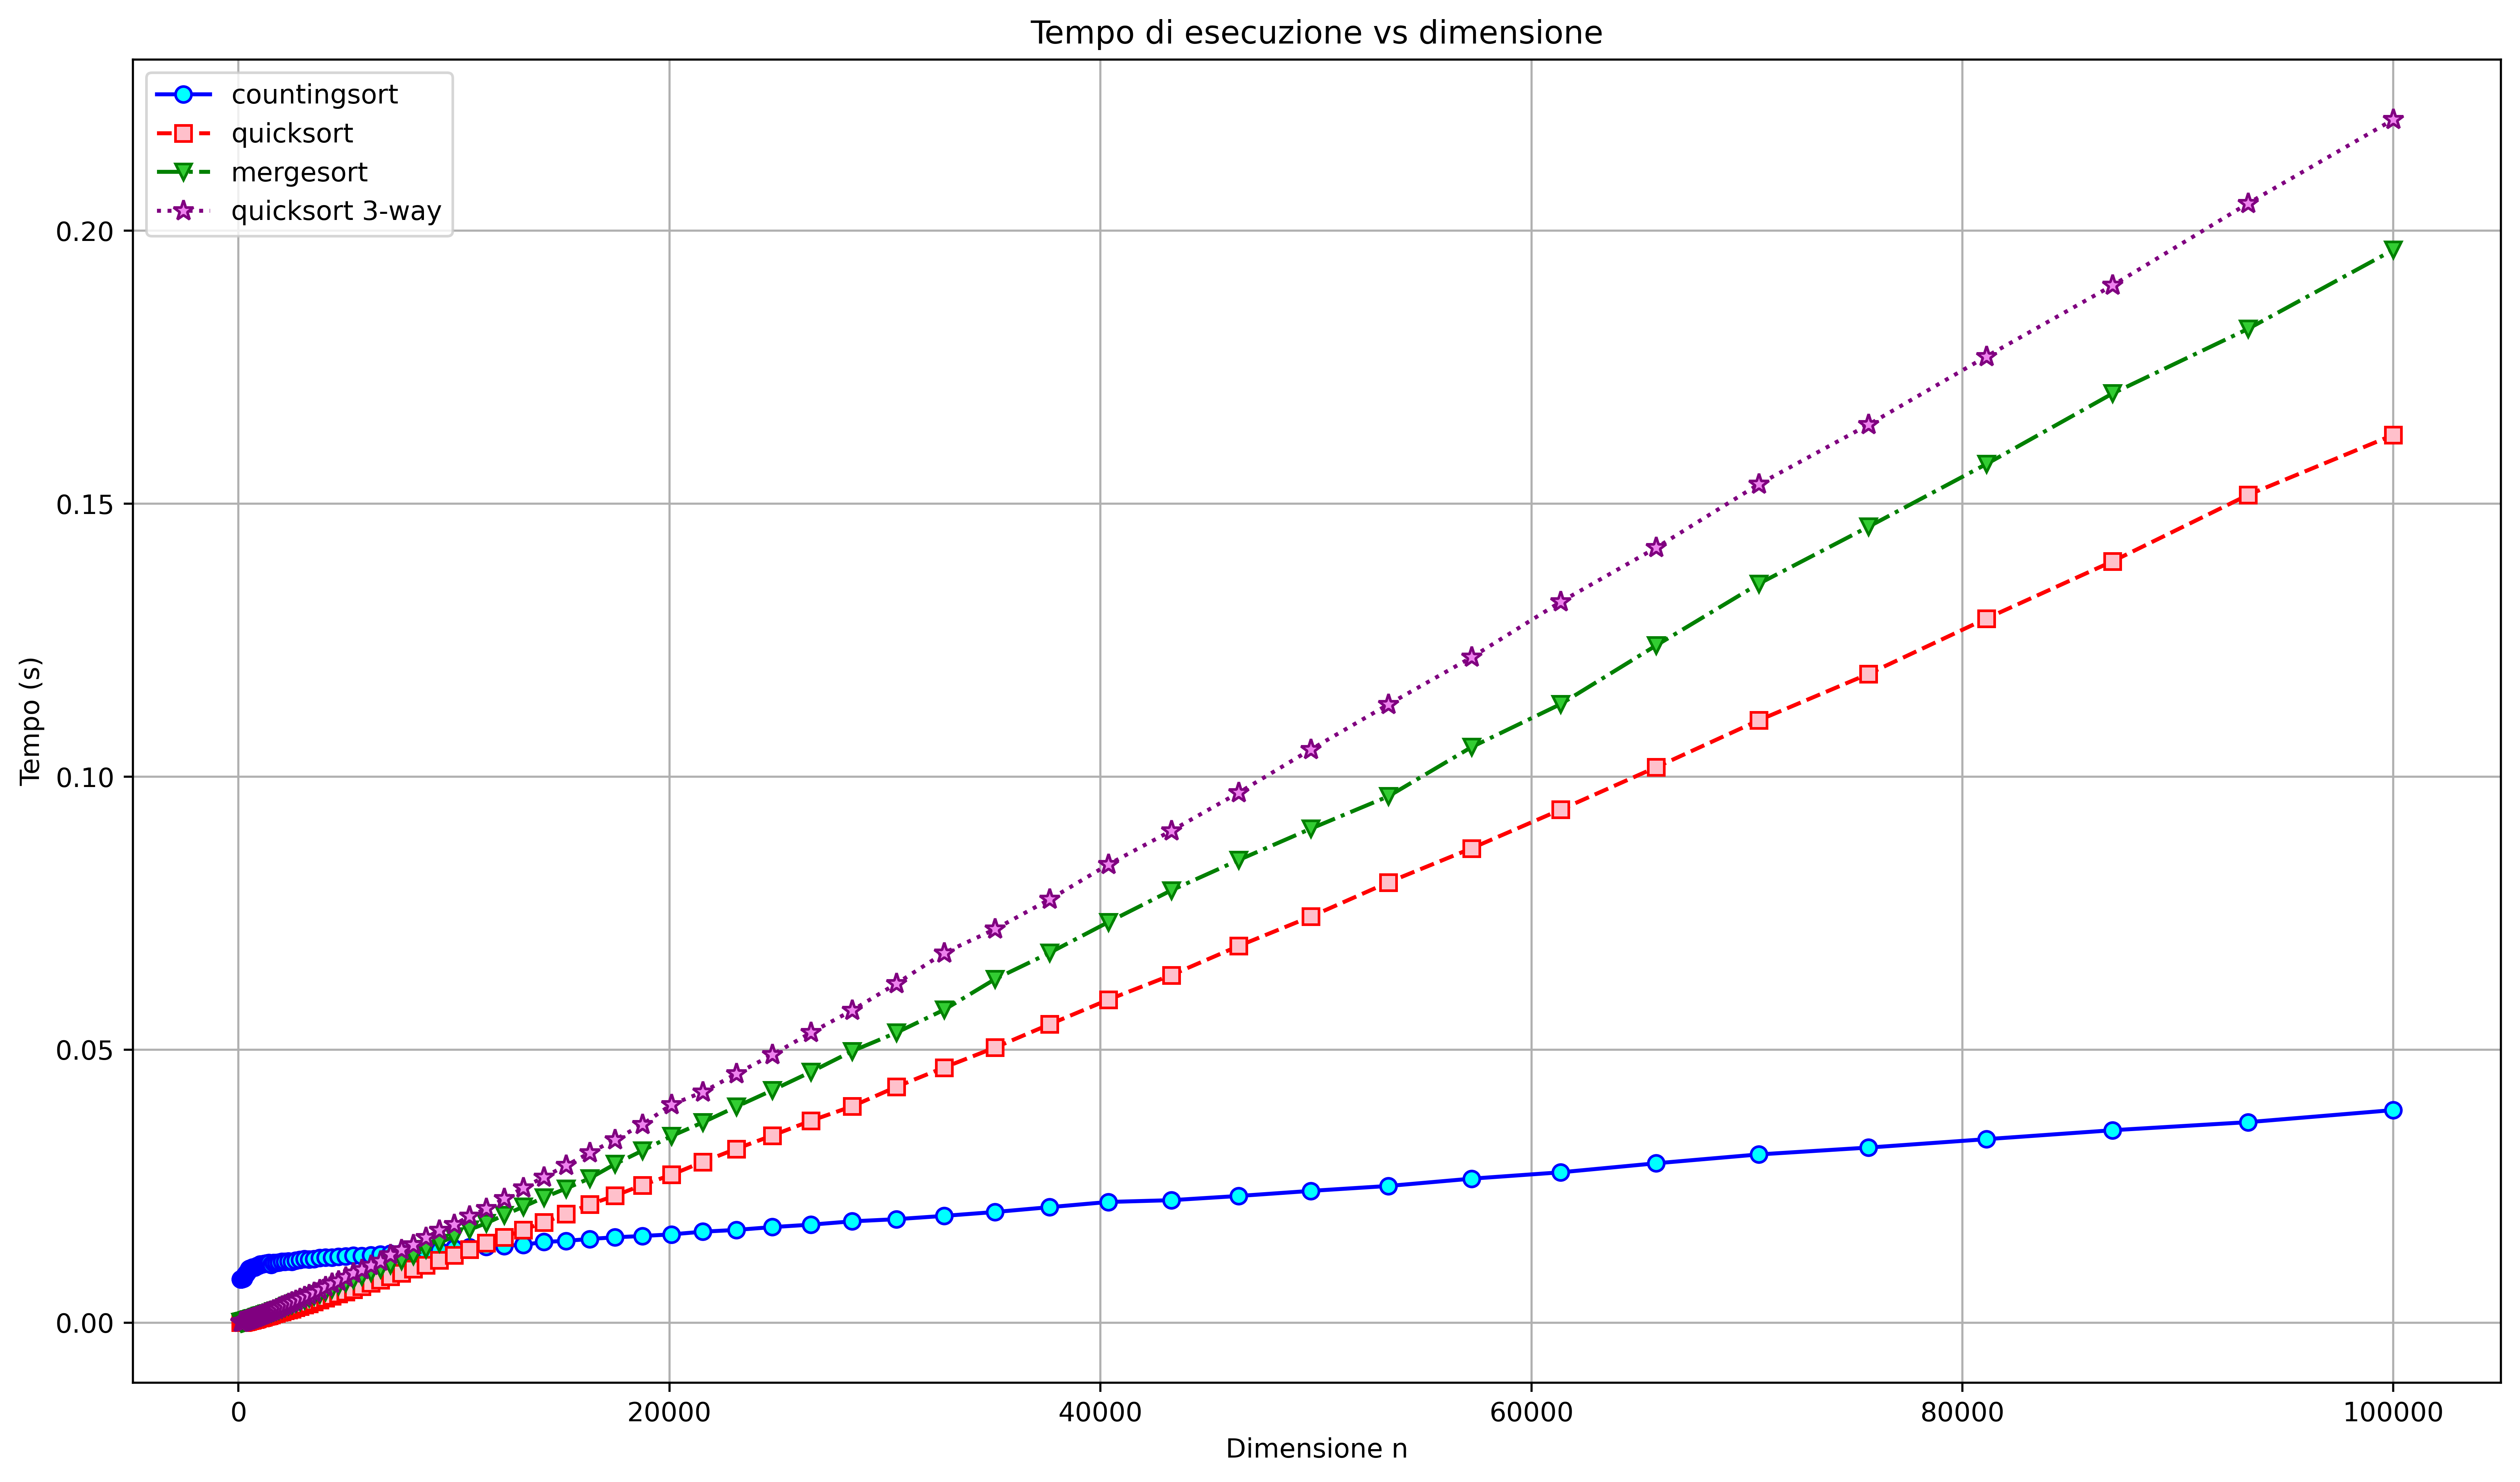
\includegraphics[width=0.95\textwidth]{Casi medi/n.png}
    \caption{Grafico in funzione della dimensione dell'array  \emph{n}}
    \label{fig:n}
\end{figure}
\begin{figure}[H]
    \centering
    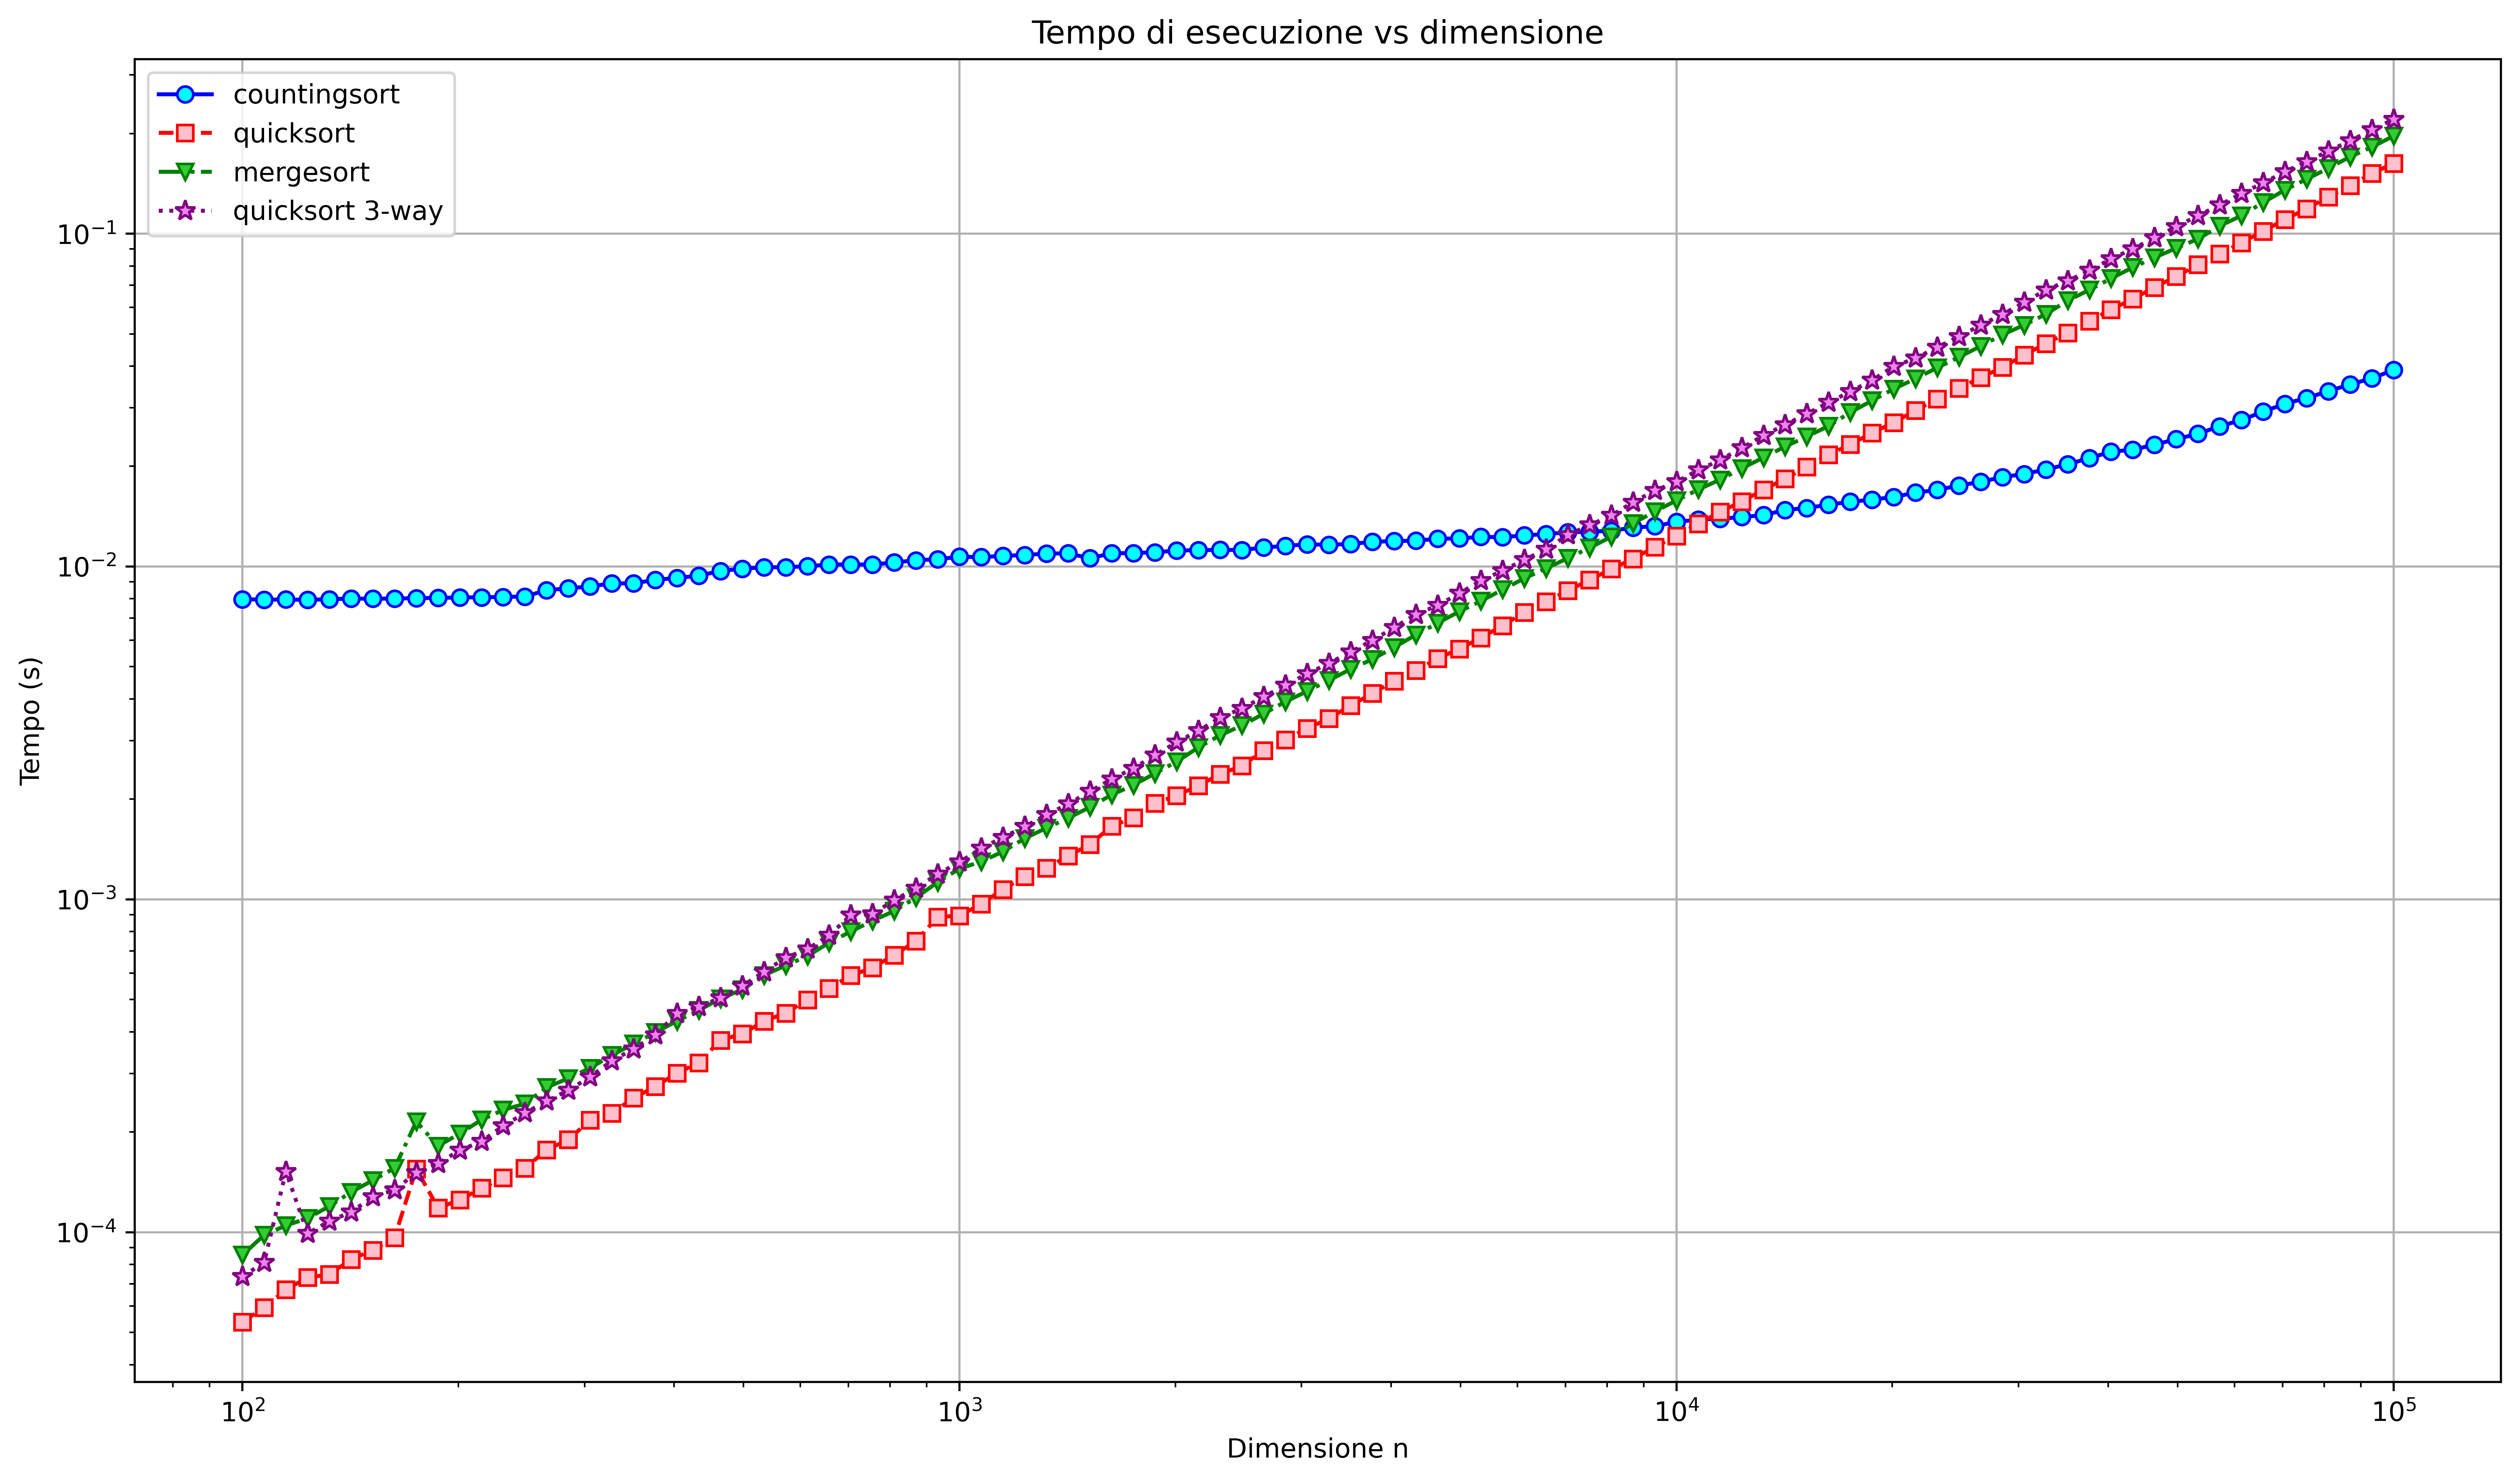
\includegraphics[width=0.95\textwidth]{Casi medi/nlog.png}
    \caption{Grafico in scala doppia logaritmica in funzione della dimensione dell'array \emph{n}}
    \label{fig:nlog}
\end{figure}

Dal grafico \emph{[Fig. 1]} si nota che l'asse delle ascisse mostra una dimensione \emph{n} crescente, mentre il range di interi è fisso a $10^5$ elementi. Sull'asse delle ordinate è riportato il tempo \emph{t} di esecuzione degli algoritmi per l'ordinamento dell'array.

Si nota che il Countingsort risulta \textbf{più lento} degli altri algoritmi quando lavoriamo con array di ordini di grandezza inferiori. All'aumentare della dimensione dell'array il Countingsort diventa notevolmente più veloce (dall'ordine di grandezza $n= 10^4$ in poi)

Questo cambiamento si spiega perché, essendo l'array costituito da interi presi da un range fisso di valori, all'aumentare della dimensione n cresce anche il numero di elementi \textbf{ripetuti}. In questa circostanza il Countingsort eccelle grazie alla sua struttura.
Inoltre la sua complessità computazionale è inferiore agli altri algoritmi, $O(n + k)$. Essendo $k \approx m$ fissato a priori, all'aumentare della dimensione la complessità degli altri tre algoritmi, $O(n log(n))$, rende i tempi di esecuzione meno vantaggiosi rispetto a quelli di Countingsort.


Gli altri tre algoritmi confrontati (Mergesort, Quicksort e Quicksort 3-way) mostrano invece prestazioni simili tra loro, dato che condividono la \textbf{stessa complessità computazionale} media di \emph{O(n log(n))}.

Nel grafico in scala doppia logaritmica \emph{[Fig. 2]} si nota molto meglio la differenza prestazionale al variare dell'ordine di grandezza della dimensione dell'array \emph{n}
\begin{itemize}
    \item per $n \leq 10^4$: Il Countingsort è molto più inefficiente degli altri algoritmi
    \item per $n > 10^4$: Il Countingsort diventa il più efficiente
    \end{itemize}
La scala doppia logaritmica ci consente di valutare per ogni \textbf{ordine di grandezza} della dimensione \emph{n} qual è l'algoritmo più efficiente.

\subsection*{Range variabile}

\begin{figure}[H]
    \centering
    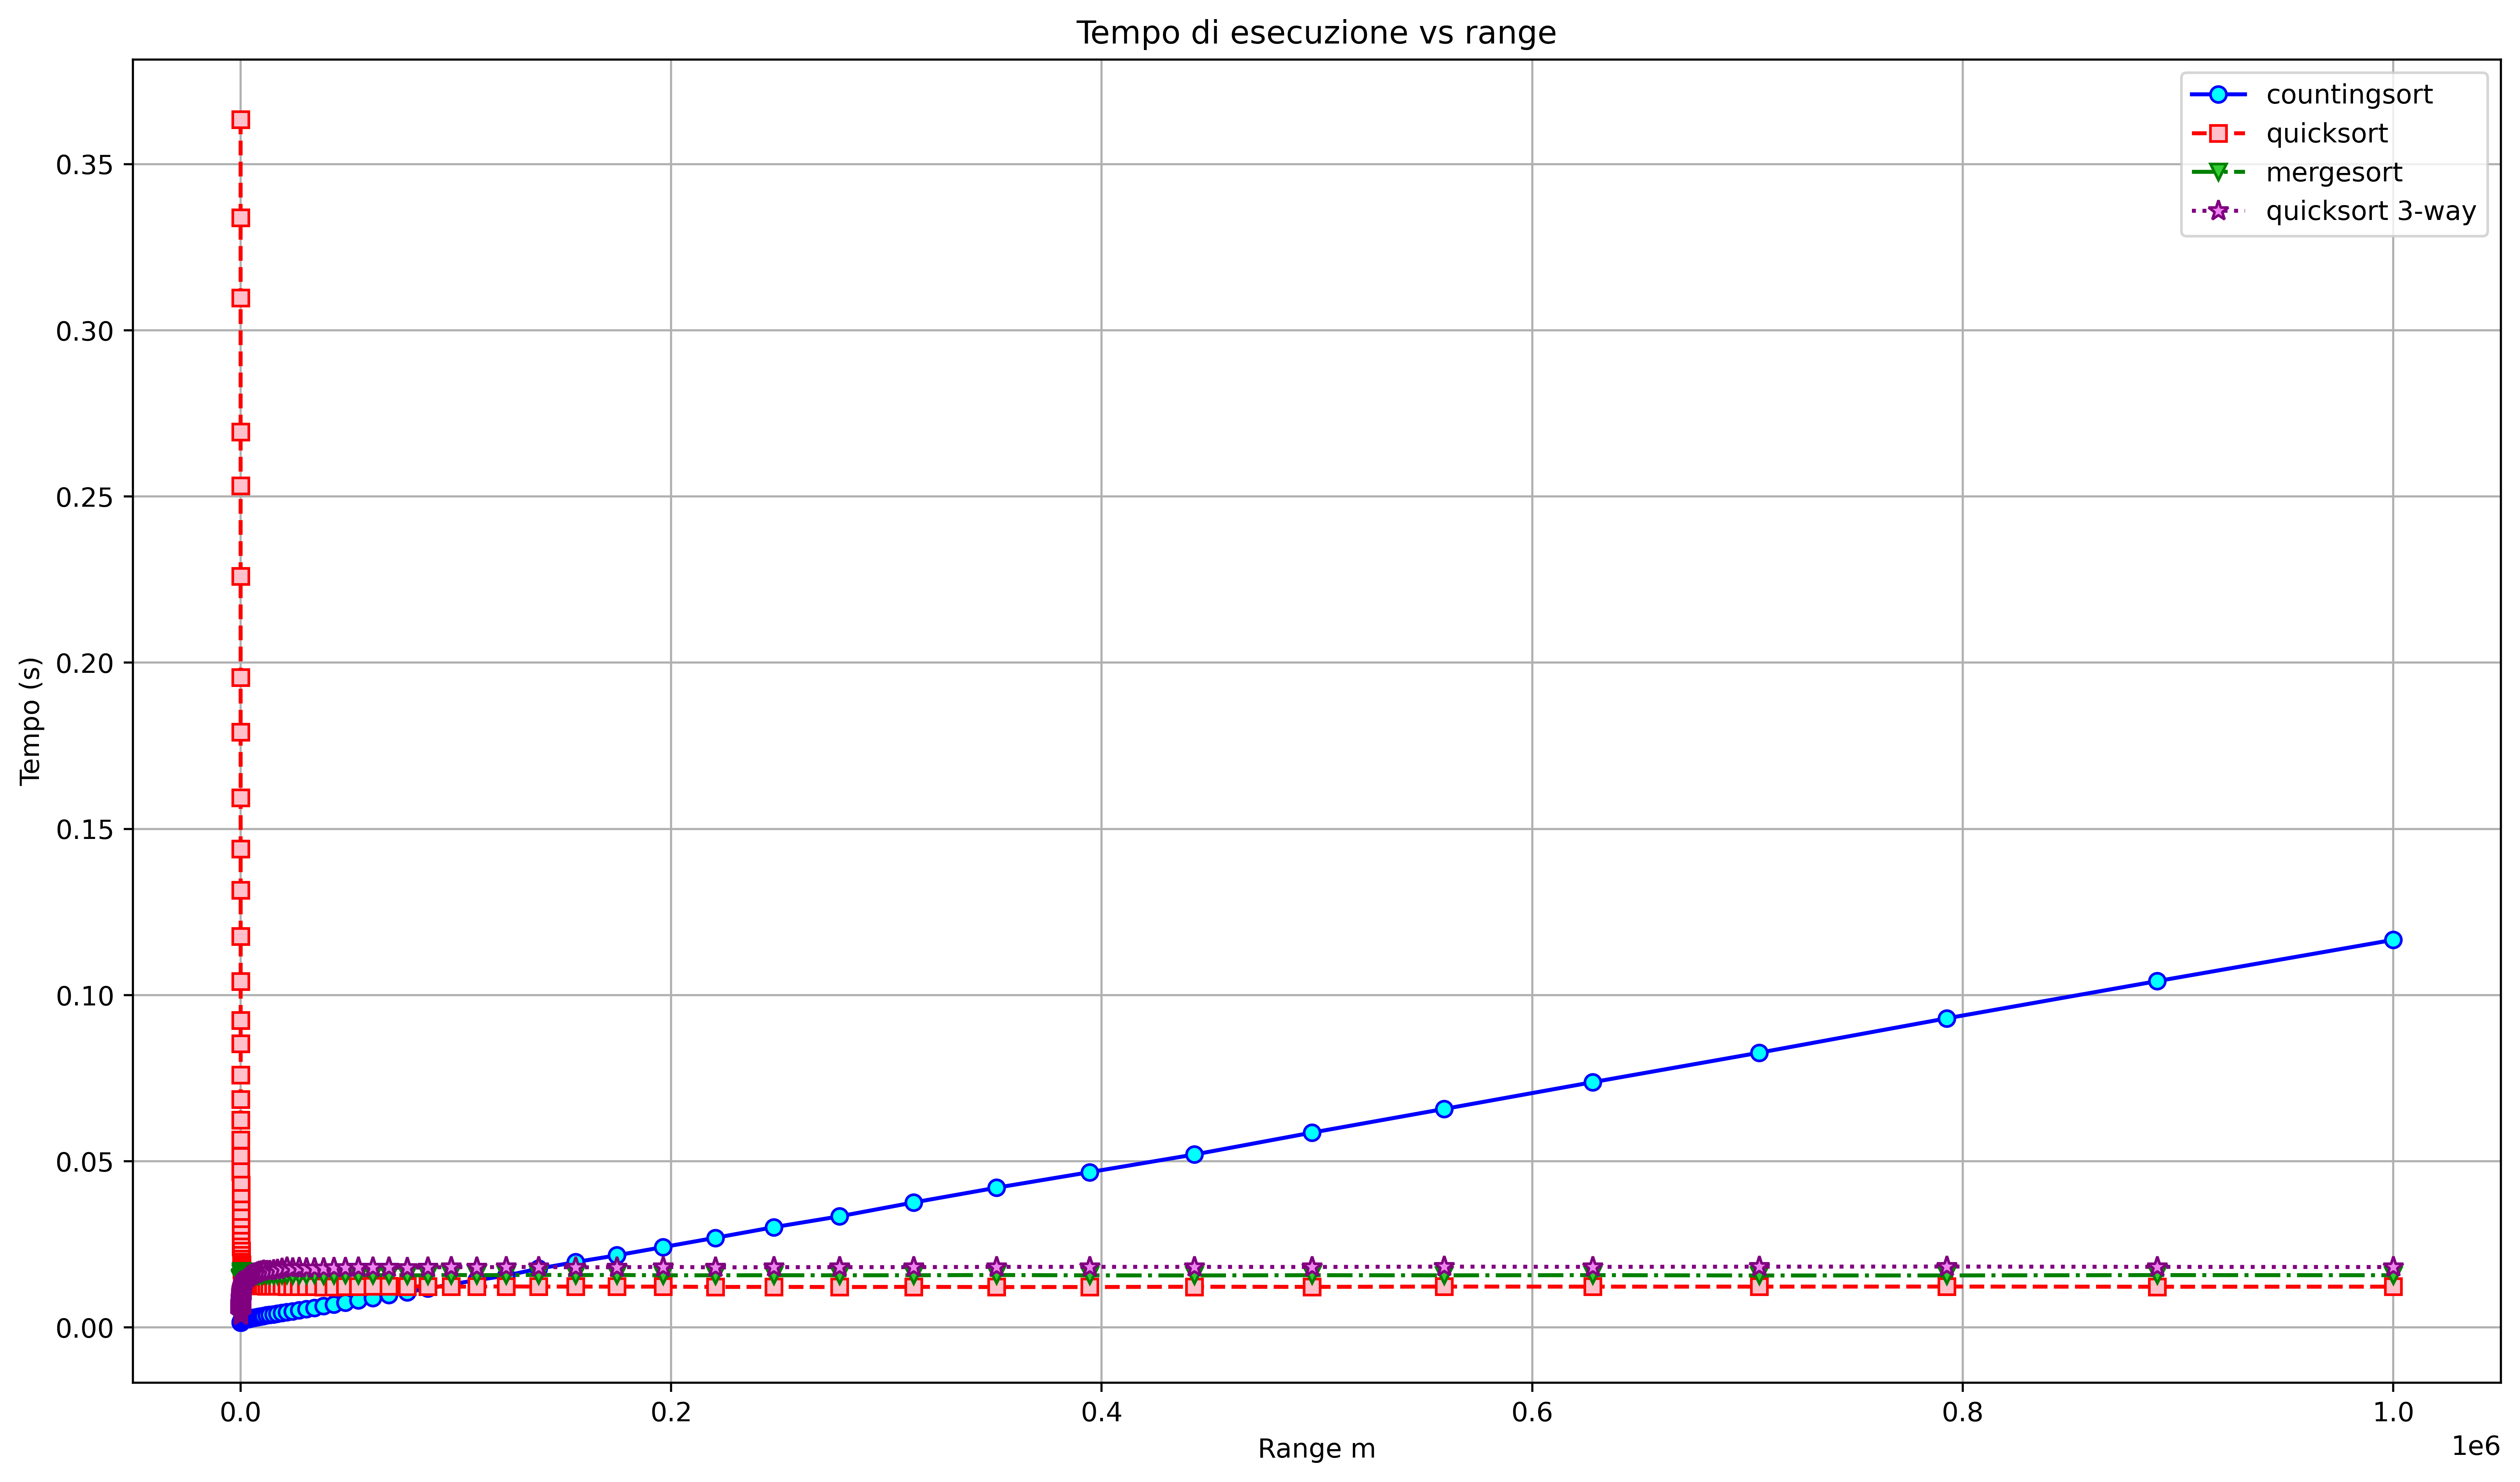
\includegraphics[width=1\textwidth]{Casi medi/m.png}
    \caption{Grafico in funzione del range di interi \emph{m}}
    \label{fig:m}
\end{figure}

Il grafico \emph{[Fig. 3]} mostra i tempi di esecuzione degli algoritmi di ordinamento al variare del range m di interi che costituiscono gli array. Gli array campione hanno dimensione \emph{n} fissata a $10^5$ elementi.

Quando il range di interi diventa più ampio, il Countingsort risulta l'algoritmo \textbf{meno efficiente}, poiché deve memorizzare un \textbf{numero maggiore di valori}. Dal grafico lineare si osserva che:
con range piccoli, il Quicksort classico è il più lento mentre il  Countingsort è il più veloce

\begin{figure}[H]
    \centering
    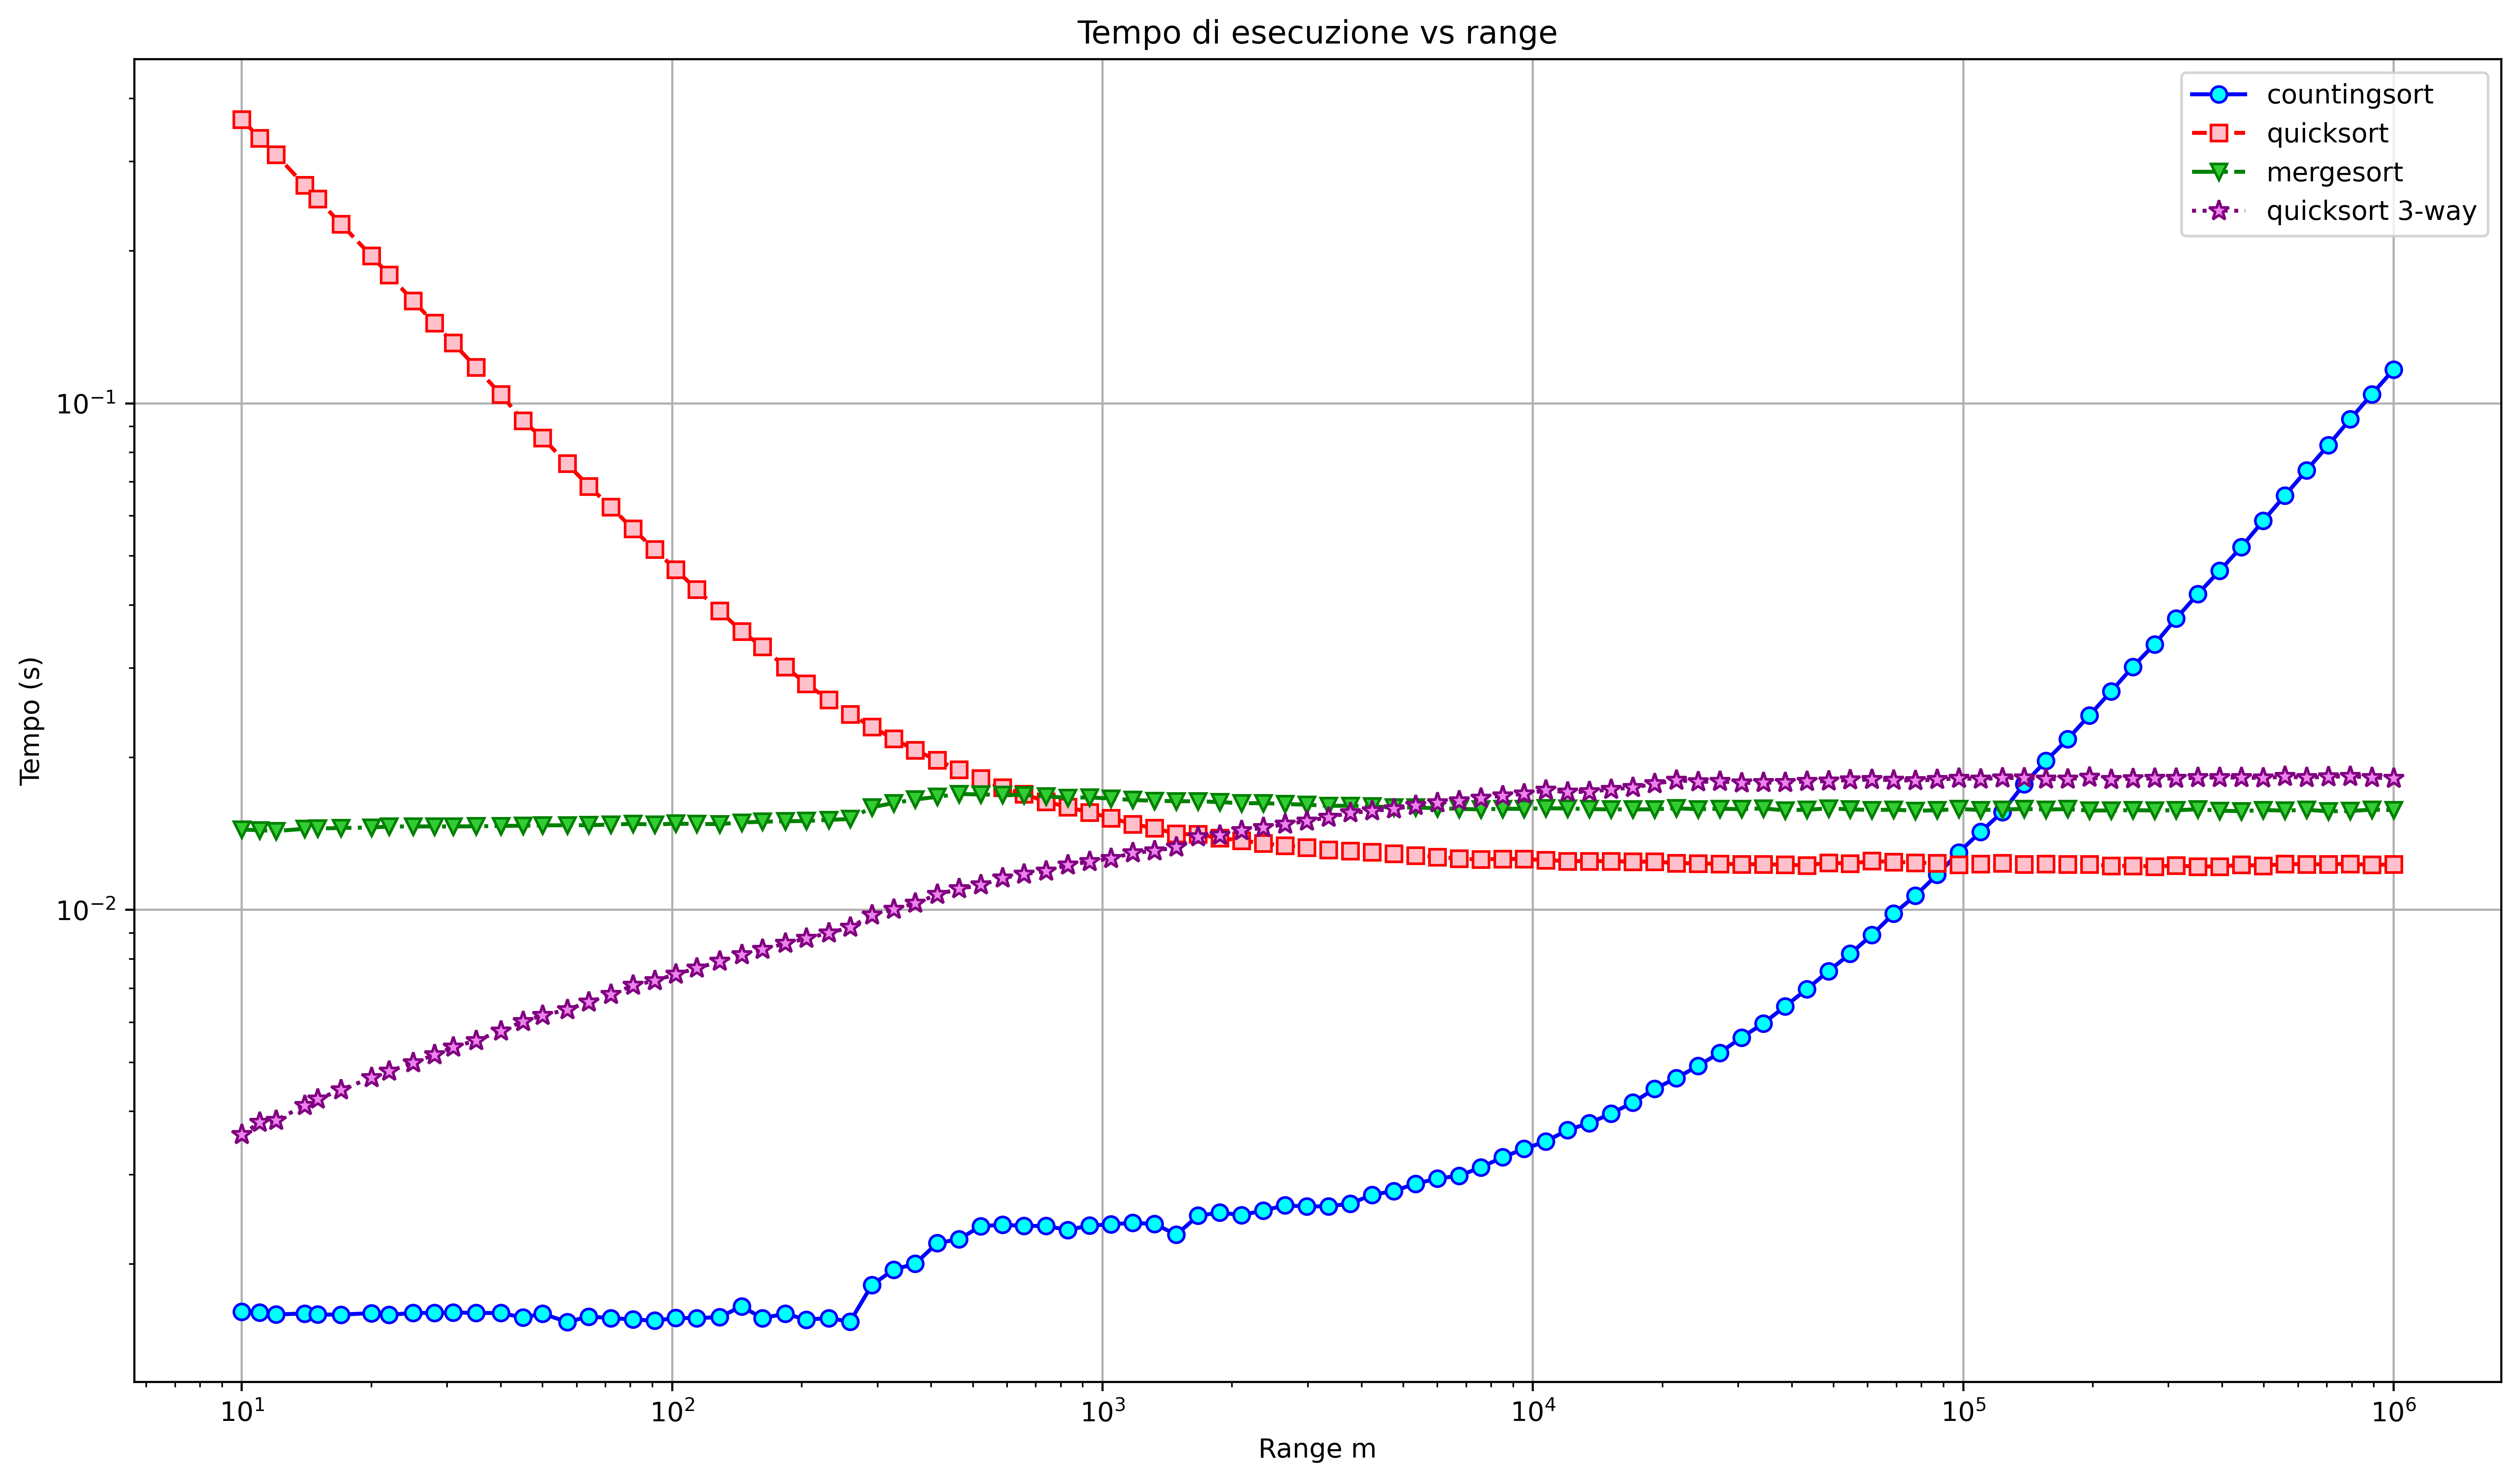
\includegraphics[width=1\textwidth]{Casi medi/mlog.png}
    \caption{Grafico in scala doppia logaritmica in funzione del range di interi \emph{m}}
    \label{fig:mlog}
\end{figure}

Nel grafico \emph{[Fig.4]} in scala doppiamente logaritmica, l'andamento risulta più chiaro:
Con il range $m < 10^3$ il Quicksort classico è il meno efficiente, poiché la presenza di \textbf{molti valori ripetuti}, tipica di range ristretti, ne penalizza le prestazioni. Il Quicksort 3-way è invece ottimale in confronto, grazie alla sua capacità di gestire efficacemente i valori ripetuti, problema che si annulla all'aumento del range valutato. 

Allo stesso modo il Countingsort si comporta meglio con range piccoli, con tempi di esecuzione minori degli altri algoritmi. Ciò accade perchè Countingsort non effettua confronti tra gli elementi dell' array, ma ne conta l'\textbf{occorrenza} di ogni valore.

Quando l'ordine di grandezza supera $10^3$ i tempi di esecuzione delle due versioni di Quicksort e di Mergesort diventano stabili, in quanto il numero di elementi ripetuti in un'array risulta \textbf{trascurabile}.

Con il range $m > 10^5$ il Countingsort diventa il più lento, poiché la crescita del range aumenta il costo di memorizzazione.
Gli altri algoritmi (Mergesort, Quicksort, Quicksort 3-way) mostrano tempi di esecuzione simili.

Il Mergesort mantiene un tempo di esecuzione \textbf{costante} all'aumentare del range \emph{m}. Questo algoritmo non è influenzato dalla presenza di valori ripetuti in quanto non fa uso di \emph{pivot} e non crea strutture legate al valore massimo e minimo presenti nell'array. Lavora solo in funzione della dimensione dell'array.
\section{Analisi dei grafici nei casi peggiori}
\label{sec:peggiori}
\subsection*{Generazione di caso peggiore}

Per analizzare i casi peggiori è stato generato un array con valori unici inseriti in ordine decrescente. Per il Countingsort si è optato per fissare il valore massimo e il valore minimo in modo da ottenere un array col massimo range possibile. Questa scelta deriva dal fatto che il caso peggiore del Countingsort si verifica quando l’array contiene elementi tutti diversi e distribuiti su un ampio intervallo di valori: in tal caso, l’algoritmo è costretto ad allocare molta memoria per gestire ciascun valore singolarmente. Per quanto riguarda Mergesort, abbiamo generato un array con un metodo chiamato \textbf{alternanza perfetta}, in cui la sequenza degli elementi è generata in modo che ogni metà abbia elementi intercalati, ovvero che si alternino elementi grandi e piccoli e l'algoritmo è costretto a confrontare ogni singolo elemento 

\subsection*{Grafici}
\begin{figure}[H]
    \centering
    
\includegraphics[width=1\textwidth]{Casi peggiori/n.png}
    \caption{Grafico in scala lineare dei casi peggiori in funzione della dimensione \emph{n}}
    \label{fig:npeggiori}
\end{figure}

Dal grafico lineare \emph{[Fig. 5]} si nota che gli algoritmi più lenti sono il Quicksort e il Quicksort 3-way, in quanto presentano una complessità nel caso peggiore pari a $O(n^2)$. Il Quicksort 3-way, eseguendo un numero maggiore di confronti, risulta essere molto più lento su array di grandi dimensioni, specialmente quando non sono presenti elementi duplicati e gli elementi sono ordinati in modo decrescente.
 Per quanto riguarda il Countingsort e il Mergesort, dal grafico lineare non si può fare una valutazione dettagliata perché le loro curve sono sovrapposte e risultano comunque molto più veloci rispetto agli altri due algoritmi.
\begin{figure}[H]
    \centering
    
\includegraphics[width=1\textwidth]{Casi peggiori/nlog.png}
    \caption{Grafico in scala doppia logaritmica dei casi peggiori in funzione della dimensione \emph{n}}
    \label{fig:nlogpeggiori}
\end{figure}


 Per analizzare meglio i comportamenti, si passa alla scala doppiamente logaritmica \emph{[Fig. 6]}, dalla quale si osserva che il CountingSort cresce molto lentamente al crescere della dimensione, ma nelle fasi iniziali, su array di piccole dimensioni, risulta essere l’algoritmo meno efficiente.

 Notiamo che due algoritmi non cambiano comportamento:
  \begin{itemize}
  \item Il Mergesort, avendo complessità $O(n log(n))$, mostra una crescita moderata. Confrontandolo con i suoi casi medi \emph{[Fig. 2]} ottiene le \textbf{stesse prestazioni}. Ciò accade perchè Mergesort divide l'array nello stesso modo in sottovettori indipendemente dai valori che lo compongono.
  \item Il Countingsort non cambia comportamento rispetto al caso medio \emph{[Fig. 2]}. Questo si può spiegare in quanto nel caso medio sono stati generati array con un range molto ampio. A causa di ciò nel caso medio è ugualmente difficile trovare tanti valori ripetuti. Il caso peggiore di Countingsort si verifica quando il range \emph{m} di interi è molto più grande della dimensione dell'array da ordinare. \textbf{Non è sensibile} alla disposizione iniziale dell'array
 \end{itemize}
\newpage

\section{Partecipanti al progetto}
\label{sec:partecipanti}
Federico Del Pup  \\
Matteo Passador   \\
Luigi Pascu       \\
Stefano Toneguzzo \\




\end{document}
